\documentclass{../../note}

\usepackage{amsthm}
\usepackage{pgfplots}
\pgfplotsset{compat=1.18}
\newtheorem{example}{Example}
\usepackage{xcolor} % For colored text
\usepackage{tikz}
\usetikzlibrary{shapes,arrows,positioning,fit,calc,matrix,decorations.pathreplacing}
\usepackage{algorithm}
\usepackage{algpseudocode}
\usepackage{listings}
\usepackage{booktabs}
\usepackage{array}
\usepackage{enumitem}
\lstset{
  basicstyle=\ttfamily\small,
  keywordstyle=\color{blue},
  commentstyle=\color{green!60!black},
  stringstyle=\color{purple},
  numbers=left,
  numberstyle=\tiny,
  numbersep=5pt,
  breaklines=true,
  frame=single,
}

\title{Exam of Datastructures}
\author{isomo}
\setlength{\parindent}{0em}
\begin{document}

\fontsize{12pt}{14.4pt}\selectfont

\maketitle


\section*{2019年}

\vspace{1cm}

\section*{一、填空题(10空,每空2分,共20分)}

\begin{enumerate}
\item 一个算法的效率可分为 \underline{\hspace{2cm}} 效率和 \underline{\hspace{2cm}} 效率。

\item 向一个长度为n的顺序表中删除第i个元素(1≤i≤n)时,需向前移动 \underline{\hspace{2cm}} 个元素。

\item 在n个结点的单链表中要删除已知结点*p,需找到它的 \underline{\hspace{2cm}} 结点,找它的后继结点没有意义。

\item 在线性结构中,第一个结点 \underline{\hspace{2cm}} 前驱结点,其余每个结点有且只有1个前驱结点;最后一个结点没有后续结点,其余每个结点有且只有 \underline{\hspace{2cm}} 个后续结点。

\item 在树形结构中,树根结点没有 \underline{\hspace{2cm}} 结点,其余每个结点有且只有 \underline{\hspace{2cm}} 个前驱结点;叶子结点没有后续结点,其余每个结点的后续可以任意多个。

\item 已知二叉树的先序和 \underline{\hspace{2cm}},不能推导出该二叉树。

\item 高度为h的完全二叉树中最多有 \underline{\hspace{2cm}} 个结点。
\end{enumerate}

\vspace{1cm}

\section*{二、单项选择题(10题, 每题2分,共20分)}

\begin{enumerate}
\item (\hspace{0.5cm}) 计算机算法指的是:

A.计算方法 B.排序方法 C.解决问题的有限运算序列 D.调度方法

\item (\hspace{0.5cm}) 链式存储的存储结构所占存储空间:

A.分两部分,一部分存放结点值,另一部分存放表示结点间关系的指针

B.只有一部分,存放结点值

C.只有一部分,存储表示结点间关系的指针

D.分两部分,一部分存放结点值,另一部分存放结点所占单元数

\item (\hspace{0.5cm}) 已知一个栈的入栈序列是1,2,3,...,n,其输出序列为p1,p2,p3,...,pn,若p1=n,则pi为:

A. i B.n=i C.n-i+1 D.不确定

\item (\hspace{0.5cm}) 判定一个栈ST(最多元素为m0)为空的条件是:

A. ST-$>$top$<>$-1 B.ST-$>$top=-1 C.ST-$>$top$<>$m0 D.ST-$>$top=m0

\item (\hspace{0.5cm}) 字符串的长度是指:

A.串中不同字符的个数 B.串中不同字母的个数

C.串中所含字符的个数 D.串中不同数字的个数

\item 下列数据结构中 (\hspace{0.5cm}) 具有先进先出(FIFO)特性, (\hspace{0.5cm}) 具有先进后出(FILO)特性。

A.线性表 B.栈 C.队列 D.广义表

\item 从逻辑上可以把数据结构分成(\hspace{0.5cm})。

A. 动态结构和静态结构 B. 顺序组织和链接组织

C. 线性结构和非线性结构 D. 基本类型和组合类型

\item 线性表若采用链式存储结构时,要求内存中可用存储单元的地址(\hspace{0.5cm})  。

A.必须连续的 B.部分地址必须连续的 C.一定是不续的 D连续不连续都可以

\item (\hspace{0.5cm}) 两个字符串相等的充要条件是:

A.两个字符串的长度相等 B.两个字符串中对应位置上的字符相等

C.同时具备(A)和(B)两个条件 D.以上答案都不对

\item 线性表L在(\hspace{0.5cm}) 情况下适于使用链表结构实现。

A. 不需修改L的结构 B. 需不断对L进行删除、插入

C. 需经常修改L中结点值 D. L中含有大量结点
\end{enumerate}



\section*{三、判断题:(10题,每题1分,共10分,在题后的括号内正确的打"√",错误的打"×")}

\begin{enumerate}
\item 算法必须具有输入、输出和正确性、安全性、易读性。 ( \hspace{0.5cm} )

\item 链表的删除算法很简单,因为当删除链中某个结点后,计算机会自动地将后续的各个单元向前移动。 ( \hspace{0.5cm} )

\item 入栈操作和入队列操作在链式存储结构上实现时不需要考虑栈溢出的情况。 ( \hspace{0.5cm} )

\item 哈夫曼树中没有度数为1的结点。 (\hspace{0.5cm})

\item 线性表的顺序存储结构优于链式存储结构。 (\hspace{0.5cm})

\item 如果某种排序算法是不稳定的,则该方法没有实际应用价值。 (\hspace{0.5cm})

\item 对于插入、删除而言,线性表的链式存储优于顺序存储。 (\hspace{0.5cm})

\item 栈和队列是操作上受限制的线性表。(\hspace{0.5cm})

\item 二叉树中所有结点,如果不存在非空左子树,则不存在非空右子树。 (\hspace{0.5cm})

\item 一个栈的输入序列是12345,则栈的输出序列不可能是12345。 (\hspace{0.5cm})
\end{enumerate}

\vspace{1cm}

\section*{四、简答题(4题,每小题5分,共20分)}

\begin{enumerate}
\item 对于一个栈,设输入项序列为A,B,C,D,E,为了得到从栈顶依次输出的序列,需要执行什么样的栈运算(push,pop)序列?哪个序列无法输出,请指出来。(1)A,B,C,D,E (2)B,C,D,E,A (3)E,A,B,C,D (4)E,D,C,B,A?

\item 请把字符串"ABCD"的所有子串写出来。

\item 说明栈与队列的异同点。

\item 请说明线性表的顺序存储结构和链式存储结构之间有什么样的区别与联系?
\end{enumerate}

\vspace{1cm}


\section*{五、综合应用题(每题15分,共30分)}

\begin{enumerate}
\item 请说明树和森林的区别,将下列由三棵树组成的森林转换为二叉树。(只要求给出转换结果,可分步骤)

\item 请说明什么是哈夫曼树?有个序列是(7,9,2,6,32,3,21,10),画出其哈夫曼树,求出其哈夫曼编码。
\end{enumerate}


\newpage

\section*{2020年}

\vspace{1cm}


\section*{一、选择题(10空,每空2分,共20分)}

\begin{enumerate}
\item 算法的五个基本特征:有输入、有输出( )。

A.可行性,可移植性和可扩充性 B.可行性,确定性和有穷性

C.确定性,有穷性和稳定性 D.易读性,稳定性和安全性

\item 设顺序线性表中有n个数据元素,则第i个位置上插入一个数据元素需要移动表中( )个数据元素;

A.n B.n-i+1 C.n-i D.n+1

\item 若已知一个栈的入栈序列是1,2,3,...,n,其输出序列为p$_1$,p$_2$,p$_3$,...,p$_n$,若p$_1$=n,则p$_i$为 。(注:p1=n意味着进栈的中间过程中没有任何元素出栈 )

A.i B.n=i C.n-i+1 D.不确定

\item ( )判定一个栈ST(最多元素为m0)为空的条件是:

A. ST-$>$top$<>$-1 B.ST-$>$top=-1 C.ST-$>$top$<>$m0 D.ST-$>$top=m0

\item 一维数组和线性表的主要区别是( )

A.前者长度固定、后者长度可变 B.前者长度固定,后者长度可变

C.前者和后者固定长度 D.后者长度固定,前者长度可变

\item 图的Depth-First Search(DFS)遍历思想实际上是二叉树( )遍历方法的推广。

A.中序遍历 B.先序遍历 C.后序遍历 D.按层次遍历

\item 用链接方式存储的队列,在进行插入运算时( )

A. 仅修改头指针 B. 头、尾指针都要修改

C. 仅修改尾指针 D.头、尾指针可能都要修改

\item 在链式队列Q中,假设队头指针为Front,队尾指针为Rear,则链队的出队操作为 ( )

(A)p=Q.front-$>$next; p-$>$next= Q.front-$>$next;

(B)p=Q.front-$>$next; Q.front-$>$next=p-$>$next;

(C)p=Q.rear-$>$next; p-$>$next= Q.rear-$>$next;

(D)p=Q-$>$next; Q-$>$next=p-$>$next;

\item 设哈夫曼树中共有n个结点,则该哈夫曼树中有( )个度数为1的结点。

A.1 B.0 C.2 D.4

\item 深度为k的完全二叉树中最少有( )个结点,最多有( )个结点。

A.2$^{k-1}$ 2$^k$-1 B.2$^k$-1 2$^k$-1 C.2$^{k-1}$ 2$^{k-1}$ D.2$^{k-1}$ 2$^k$+1
\end{enumerate}


\vspace{1cm}


\section*{二、填空题(8题, 每空2分,共20分)}

\begin{enumerate}
\item 线性表的五个基本运算有插入、删除、修改,\underline{\hspace{2cm}},\underline{\hspace{2cm}}。

\item 设指针变量q指向单链表中结点A,若要在单链表结点p之后插入结点A,则需要修改指针的操作序列为\underline{\hspace{2cm}},\underline{\hspace{2cm}}。

\item 在树形结构中,树根结点没有\underline{\hspace{2cm}}结点,其余每个结点有且只有1个直接前驱结点,叶子结点没有\underline{\hspace{2cm}}结点,其余每个结点的直接后继结点可以有\underline{\hspace{2cm}}。

\item 设有向图中完全有n个顶点,则该完全有向图中最多有\underline{\hspace{2cm}}条有向边。

\item 线性结构中\underline{\hspace{2cm}}具有先进先出(FIFO)特性,\underline{\hspace{2cm}}具有先进后出(FILO)特性。

\item 设顺序线性表中有n个数据元素,则第i个位置上删除一个数据元素需要移动表中\underline{\hspace{2cm}}个数据元素;

\item 分析下面算法(程序段),该算法的时间复杂度是\underline{\hspace{2cm}}。

for (i=0;i$<$n;i++)

\hspace{1cm}for (j=0; j$<$i; j++)

\hspace{2cm}A[i][j]=0;
\end{enumerate}


\vspace{1cm}


\section*{三、判断题:(10题,每题1分,共10分,在题后的括号内正确的打"√",错误的打"×")}

\begin{enumerate}
\item 算法必须具有输入、输出和正确性、安全性、易读性。 ( \hspace{0.5cm} )

\item 链表的删除算法很简单,因为当删除链中某个结点后,计算机会自动地将后续的各个单元向前移动。 ( \hspace{0.5cm} )

\item 入栈操作和入队列操作在链式存储结构上实现时不需要考虑栈溢出的情况。 ( \hspace{0.5cm} )

\item 哈夫曼树中没有度数为1的结点。 ( \hspace{0.5cm} )

\item 稀疏图是指为零元素非常少的矩阵。 ( \hspace{0.5cm} )

\item 对于插入、删除而言,线性表的链式存储优于顺序存储。 ( \hspace{0.5cm} )

\item 一棵深度为5的满二叉树的结点总数为32。 ( \hspace{0.5cm} )

\item 由二叉树的先序序列和后序序列可以唯一确定一颗二叉树。 ( \hspace{0.5cm} )

\item 一个栈的输入序列是12345,则栈的输出序列不可能是12345。 ( \hspace{0.5cm} )
\end{enumerate}

\vspace{1cm}


\section*{四、简答题(4题,每小题5分,共20分)}

\begin{enumerate}
\item 什么是算法,算法的特性是什么(要求描述每个特性的的含义)?

\item 什么是栈,栈的特点是什么?

\item 试述折半查找的过程。

\item 试述冒泡排序的过程。
\end{enumerate}

\vspace{1cm}


\section*{五、综合应用题(每题10分,共30分)}

\begin{enumerate}
\item 已知二叉树的遍历序列如下,先画出这两棵二叉树,然后分别写出它们的\textbf{先序序列}和\textbf{后序序列}。

(1)先序序列:ABCDEFGH 中序序列:CBEDFAGH

请写出该二叉树的后序遍历序列。

(2) 后序序列为DCEGBFHKJIA,中序序列为DCBGEAHFIJK

请写出该二叉树的先序遍历序列。

\item 解答下列两个问题。

(1) 下图的无向带权图,从顶点a开始按普里姆算法求其最小生成树。(\textbf{给出求解过程})

\begin{figure}[h]
\centering
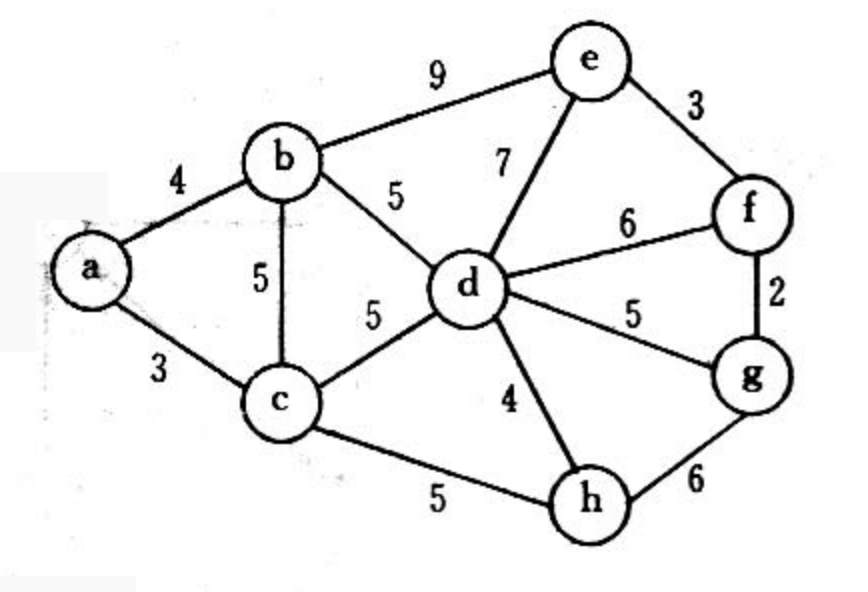
\includegraphics[width=0.5\textwidth]{./graph.png}
\caption{Prim算法示例}
\end{figure}

(2) 写出从顶点1出发的两种拓扑序列(\textbf{任意两种即可,答案不唯一})

\begin{figure}[h]
\centering
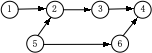
\includegraphics[width=0.5\textwidth]{./graph_tree.png}
\caption{拓扑排序示例}
\end{figure}

\item 请说明什么是哈夫曼树?有个序列是(12,4,5,6,1,2),画出其哈夫曼树,并求出其带权路径长度WPL。
\end{enumerate}

\vspace{1cm}

\end{document}
